
\section{Rozbor problému}
\label{kap:1}

\subsection{SCARA - kinematická štruktúra}
\label{kap:1.1}

\subsubsection{2 stupne voľnosti}
\label{kap:1.1.1}

\subsubsection{3 stupne voľnosti}
\label{kap:1.1.2}

\subsection{Algoritmy plánovania trajektórie}
\label{kap:1.2}
 
\subsubsection{RRT}
\label{kap:1.2.1}

Algoritmus RRT – z anglického Rapidly-exploring Random Tree, by sa dal do slovenčiny preložiť ako rýchlo rastúci náhodný strom. Algoritmus je v oblasti robotiky veľmi rozšírení a obľúbený vďaka svojej schopnosti rýchlo prehľadávať vysoko dimenzionálny konfiguračný priestor, v ktorom zohľadňuje prekážky v priestore ako aj dynamiku telesa. \newline
Ide o algoritmus založený na prehľadávaní konfiguračného priestoru $C$ , kde sa v iteráciách vytvárajú náhodné uzly - $q$, ktorých spájaním vznikajú nové potenciálne cesty. Každý uzol $q$ reprezentuje pozíciu a orientáciu telesa v 2D alebo 3D priestore [1]. Pri plánovaní trajektórie je generovaný kontinuálny rad uzlov (obr. \ref{OBRAZOK 1.2.1}), ktorý začína v počiatočnom stave $q_{init}$,  a postupne sa rozrastá až dosiahne koncový stav $q_{goal}$.  Generovanie stromu prebieha v iteráciách kedy sa vždy vygeneruje náhodná konfigurácia $q_{rand}$ a nájde sa k nej najbližší uzol patriaci stromu. Od daného uzla je následne vo vzialenosti v od uzla $q_{nearest}$ vytvorený nový uzol $q_{new}$. Proces rozrastania stromu sa končí v momente ak sa $q_{new}$  nachádza v okolí cieľovej konfigurácie $q_{goal}$, ktoré je definované vzdialenosťou $d$. Ak neuvažujeme voľný konfiguračný priestor $C_{free}$ treba v procese generovania taktiež overovať kolíziu s danými prekážkami v priestore - $C_{obs}$. Novo generovaný uzol stromu sa nesmie nachádzať v priestore prekážky - $C_{obs}$, a ani cesta medzi dvoma susednými uzlami nesmie kolidovať s prekážkou. Pokiaľ uzol spĺňa tieto podmienky, je zaradený do štruktúry stromu, v opačnom prípade je vyradený a proces pokračuje ďalej.

\begin{figure}[h]
	\centering
	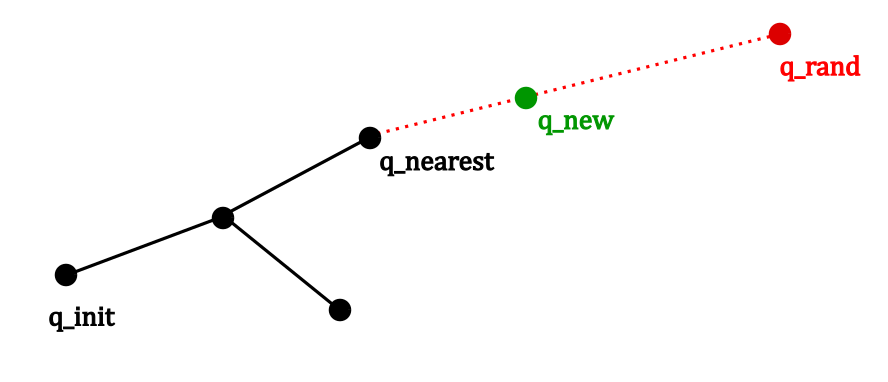
\includegraphics[width=120mm]{img/RRT1.png}
	\caption{Vizualizácia princípu RRT algoritmu }\label{OBRAZOK 1.2.1} 
\end{figure}  

Ide o neoptimálne riešenie, keďže body v konfiguračnom priestore sú generované náhodne a výsledný tvar trajektórie vzniká ako najkratšia cesta medzi nami vygenerovanými bodmi. Na zlepšenie trajektórie existuje viacero možností, ktoré ponúkajú suboptimálne riešenia problému, jedným z nich je napríklad RRT*.  

\subsubsection{RRT*}
\label{kap:1.2.2}

Jedná sa o modifikáciu RRT algoritmu, ktorej cieľom je v porovnaní s pôvodným RRT nájsť kratšiu trajektóriu. Hlavnou úpravou oproti jednoduchému RRT algoritmu je výpočet vzdialenosti z počiatočného do aktuálneho uzlu a následné overenie, či neexistuje v okolí uzol, ktorého vzdialenosť by bola menšia ako vzdialenosť momentálneho prepojenia. Ak táto situácia nastane, algoritmus vyberie prepojenie uzlov , ktoré vytvoria kratšiu trasu. Algoritmy sa tiež líšia ukončovacou podmienkou, kde pre RRT* je určený jasný počet iterácií. Od počtu iterácií závisí výsledný tvar trajektórie, kde so zvyšujúcim sa počtom je algoritmus schopný nájsť kratšie a plynulejšie trasy (obr. \ref{OBRAZOK 1.2.2}).

\begin{figure}[h]
	\centering
	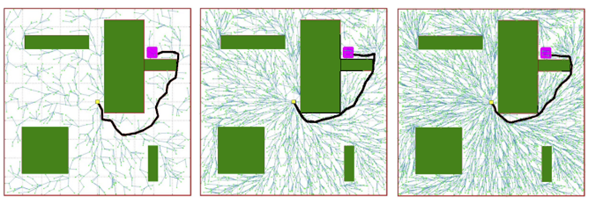
\includegraphics[width=160mm]{img/RRT2.png}
	\caption{Vplyv počtu iterácií na výslednú trajektóriu \cite{}}\label{OBRAZOK 1.2.2} 
\end{figure} 

\subsubsection{RRT - connect (prepojený)}
\label{kap:1.2.3}
Ďalšou z modifikácií je algoritmus RRT Connect (spojenie). Algoritmus v procese rozširovania stromovej štruktúry vytvára 2 stromy z počiatočnej a koncovej konfigurácie, ktoré sa šíria v konfiguračnom priestore až dokým nedôjde k ich spojeniu a tak vytvoreniu cesty (obr. \ref{OBRAZOK 1.2.3}).

\begin{figure}[h]
	\centering
	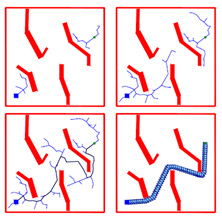
\includegraphics[width=70mm]{img/RRT-connect.png}
	\caption{Prepojenie 2 stromov \cite{}}\label{OBRAZOK 1.2.3} 
\end{figure} 

\subsubsection{Potenciálové pole}
\label{kap:1.2.4}

Plánovanie trajektórie na základe potenciálového poľa využíva koncept odpudivých a príťažlivých polí. Príťažlivé pole generuje veľmi nízke hodnoty so stredom v cieľovom bode, ktoré sa so zväčšujúcou sa vzdialenosťou od cieľa zvyšujú. Odpudivé pole zase naopak generuje veľmi vysoké hodnoty v okolí prekážok v priestore. Kombináciou daných dvoch polí dostávame tzv. potenciálové pole (obr. \ref{OBRAZOK 1.2.4}) so silným sklonom ku cieľu tak aby generovaná trajektória mala tendenciu vyhýbať sa prekážkam.

\begin{figure}[h]
	\centering
	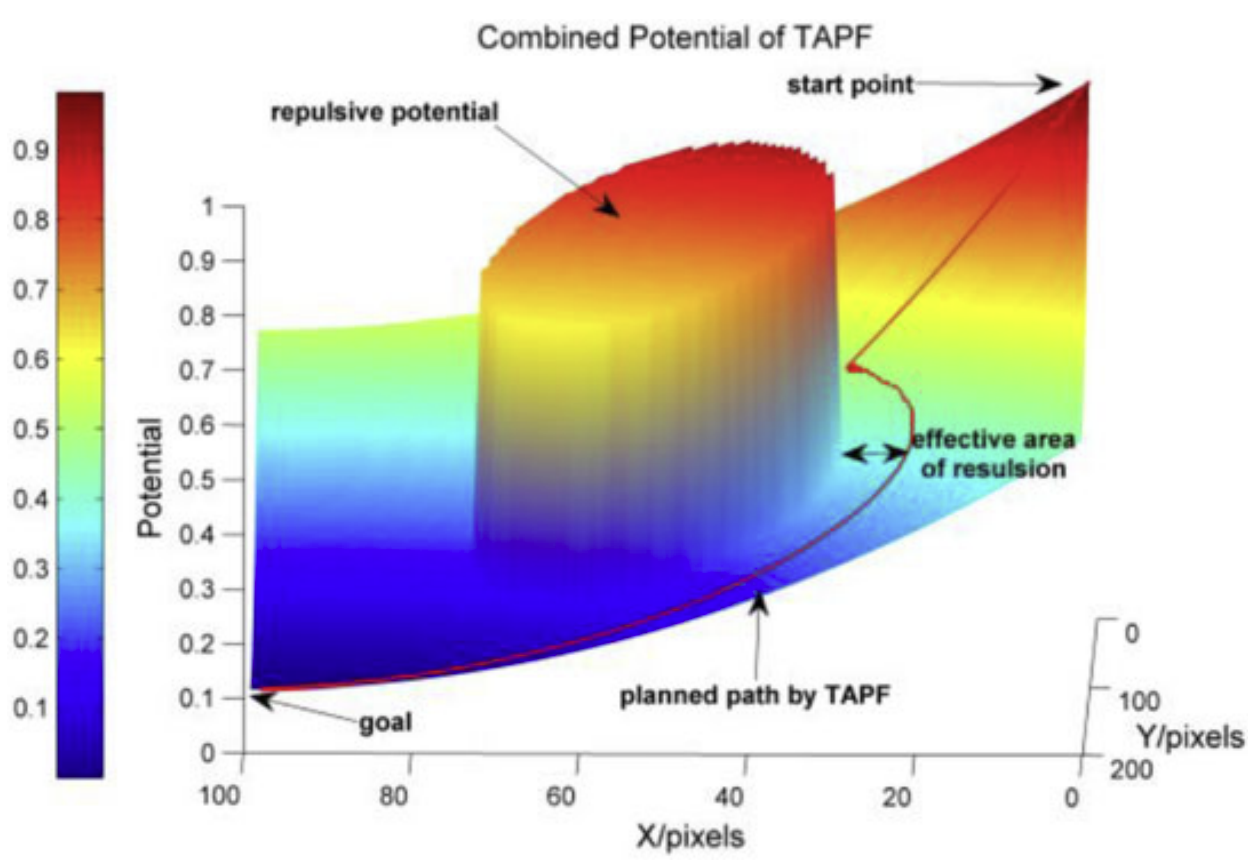
\includegraphics[width=100mm]{img/Potencialove_pole2.png}
	\caption{Potenciálové pole \cite{}}\label{OBRAZOK 1.2.4} 
\end{figure} 